\documentclass[12pt,a4paper,notitlepage]{article}
\usepackage[utf8]{inputenc}
\usepackage{amsmath}
\usepackage{wrapfig, blindtext}
\usepackage{amsfonts}
\usepackage{longtable}
\usepackage{amssymb}
\usepackage{graphicx}
\usepackage[a4paper, left=.6in,right=.6in,top=.8in,bottom=.8in,]{geometry}
\usepackage{tabularx,ragged2e,booktabs,caption}
\usepackage{setspace}
\setstretch{1.5}
\usepackage{tabularx, booktabs}
\usepackage{dcolumn} 
  \newcolumntype{d}[1]{D{.}{.}{#1}}    
\newcolumntype{Y}{>{\centering\arraybackslash}X}
\usepackage[T1]{fontenc}
\usepackage{epigraph}
\usepackage{url}
\usepackage[round,sort]{natbib}
\newcommand{\source}[1]{\caption*{\footnotesize Source: {#1}} }
\usepackage{float}
\usepackage[section]{placeins}
\usepackage{ctable}
\newcolumntype{?}{!{\vrule width 2pt}}
  \newcolumntype{d}[1]{D{.}{.}{#1}}  

\begin{document}
\title{Were mercantilist trade wars "good, and easy to win"? \\
Lessons from the Second Hundred Years War}
\author{
  Guillaume Daudin \\ Université Paris-Dauphine \\guillaume.daudin@dauphine.psl.eu		
  \and
  Elisa Tirindelli\footnote{This paper is not part of my PhD dissertation. It is the continuation of my master's thesis which I am now trying to publish with my previous supervisor, as my co-author. My present supervisor in Trinity College is not involved in this project.} \\ Trinity College Dublin  \\ tirindee@tcd.ie
}
\date{}
\maketitle

%\section*{Abstract}

\epigraph{Savez-vous Messieurs ce qu’est une bataille navale ? On se rencontre, on se salue, on se canonne et la mer n’en reste pas moins salée.}{Maurepas, Navy Minister of Louis  \textsc{xv}, 1718-1748}

What made mercantilist warfare effective in its own terms, i.e. by crippling trade of defeated powers?
Our paper explores the Anglo-French experience during the eighteenth century and disentangles the effects of the strategies implemented to curtail enemy's trade.
Thanks to a new database of French trade statistics\footnote{http://toflit18.hypotheses.org}, we were able to analyse the impact of a prolonged period of mercantilist warfare, not only on aggregate trade, but also on its structure, narrowing down our analysis to fourteen distinct product categories.
We compute a war loss function for French trade.
We then quantify the disruptive effects of different elements, such as naval supremacy, colony loss, policy towards neutral countries, activities of privateers and British Navy and Army budget.
As far as aggregate trade is concerned, we could not identify a specific cause that systematically explains success in inflicting major post-war losses.
However we identify a clear link between long lasting changes in trade structure and French trade losses. \\
%We then analyse the link between warfare strategies and permanence of changes in trade composition.\\

%%I am not sure about the laste sentence. Do you have something in mind ?
\cite{jefferson_letter_1823} famously noticed that European nations \textit{were nations of eternal war}.
Indeed, from 1700 to 1825, two years out of three experienced conflict between major European powers \citep{roser_war_2016}.
Rivalry between Great-Britain and France was central, so much as the period between 1688 to 1815 was called the ``Second Hundred Years War''.
Mercantile rivalry was an important motivation of French wars (\cite{wallerstein_modern_1980, crouzet_guerre_2008}).
Each nation was jealous of the other's commercial success.
The British believed war was a good way to curtail French trade.
The French believed it could be a good way to curtail British trade, but were more wary of wars because they did not have much naval success.
It is not obvious whether any of the long list of wars between France and Britain after the death of Louis XIV - War of the Polish Succession (1733-1738) (little naval hostilities), War of the Austrian Succession (1740-1748, where naval hostilities started in 1744), Seven Years' War (1756–1763) and the War of American independence (1775–1783, where French involvement started in 1778) - achieved their mercantile goal effectively.
Figure \ref{FrBritTrade} shows that French trade, despite a decrease in wartime, was recovering quite fast after each of these four wars.
French Revolutionary Wars (1792–1802) and Napoleonic Wars (1803–1815) were much more decisive in that respect.
\begin{figure}
\caption{French, British trade and Anglo-French wars}
\centering
\includegraphics[scale=.7]{"Total silver trade FR GB".pdf}
\source{French trade up to 1821: \cite{daudin_toflit18_????}. French trade 1822-1840: \cite{federico_world_2016} / \cite{dedinger_exploring_2017},

England/British trade up to 1800: \cite{deane_british_1969}. UK trade from 1801 to 1840: \cite{federico_world_2016} / \cite{dedinger_exploring_2017},

Livre tournois silver value: \cite{de_wailly_memoire_1857} and \cite{hoffman_priceless_2000}; Pound sterling silver value: \cite{clark_england_1209-1914_2006} and \cite{jastram_silver_1981}}
\label{FrBritTrade}
\end{figure}
Computing a loss function for French trade, however, reveals a slightly different picture.
Loss is defined as the percentage loss of trade compared to past peace time trend:
\begin{equation*}
Loss = \frac{Expected \> value \> based \> on \>past \> peace \>trend - Observed \> value}{Expected \> value \> based \> on \>past \> peace \>trend}
\end{equation*}
Figure \ref{annual_loss_function} shows the annual loss function for the period of interest. Figure \ref{mean_loss_function} shows the mean loss function by peace or war period.
\begin{figure}[H]
	\begin{minipage}[b]{0.45\linewidth}
		\caption{Annual Loss Function}
		\centering
		\label{annual_loss_function}
		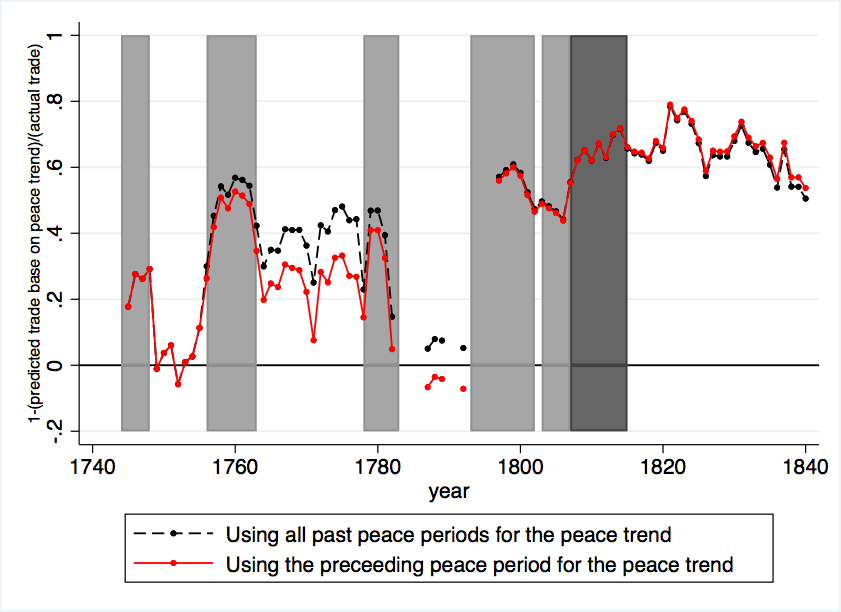
\includegraphics[scale=.3]		{Annual_loss_function.png}
	\end{minipage}
	 \hspace{0.5cm}
     \begin{minipage}[b]{0.45\linewidth}
	\caption{Mean Loss Function}
	\label{mean_loss_function}
	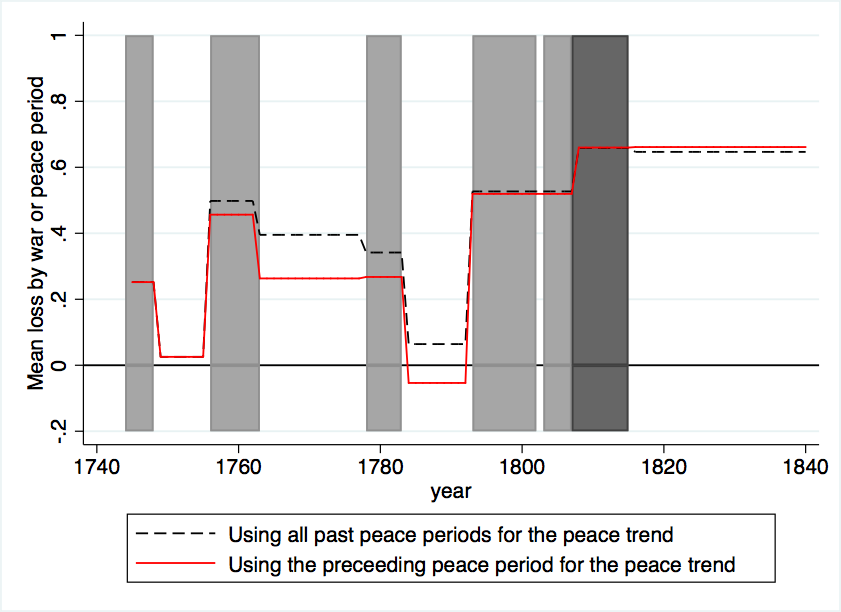
\includegraphics[scale=.3]{Mean_loss_function.png}
	\end{minipage}
\end{figure}
These two figures show that the peace percentage loss of the Seven Years Wars and that of the Napoleonic Wars, were comparable to wartime loss, as opposed to faster recoveries in other post-war periods.
What made these wars so effective in terms of trade disruption?
How were they different from other similar wars in the same century? \\~\\
In light of the recent events - the trade war between US and China for instance - it is important to understand the effects of wars and trade wars in general. We are doing so from an historical perspective, because we believe that understanding the geopolitical history of the eighteenth and nineteenth century and the globalization/deglobalization cycle from the 1490s to the 1840s can shed light on mechanisms still in place nowadays.  \\~\\
To answer this question we attempt to quantify the impact of the different factors at play. \\
Naval supremacy was an important determinant of efficacy of a trade conflict.
British naval supremacy over France meant that Britain could blockade French ports and capture French ships in a more efficient way.
To produce a yearly measure of naval supremacy, we use the number of warships available to France, France and its allies, Great Britain, Great Britain and its allies and neutral as provided in \cite{modelski1988seapower}.
We find that the most favourable war for France and its allies, in terms of naval supremacy, was the Seven Years War, which, according to the loss function, was one of the toughest in terms of forgone trade.
This suggests that naval supremacy is not a sufficient explanation. \\ 
Another possible factor is colony loss. French trade was relying heavily on import and re-export of colonial goods, especially sugar from Saint Domingue, which was lost at the end of the 18th century. We construct a measure to account for this.
This measure equals 1 when France had all its colonies, and gets reduced by an amount proportional to the value of forgone trade whenever a colony is lost.
Colonial losses were the largest during the Revolutionary \& Napoleoncic Wars, but it cannot explain the loss in trade during the Seven Years War. \\
Finally, we explore the hypothesis of the role of neutral trade during conflicts. 
The way the Neutrals were treated was important in British eandeavors to destroy French trade, as the merchants from France allied countries used a number of devices to "hide" their cargo as neutral cargo, and continue trade (see \citep{carriere1973negociants}, \cite{schnakenbourg2013guerre}). 
During the century, Great Britain tried to close off these devices to prevent French trade to continue thanks to neutral shipping.
In 1756, during Seven Years War, the British tried to reduce French trade on neutral ships by introducing the \textit{Doctrine of Continuous Voyage} along with the \textit{Rule of War of 1756}, that stated that the very beginning of the journey and the very end should be taken into account to determine the nationality of the cargo.
They also claimed and exercised the right to seize neutral shipping to look for contraband.
The situation for neutral trade was not very different during the Revolutionnary \& Napoleonic wars, as France itself became more and more hostile to neutral shipping as a way to try and isolate Great Britain. Even without a proper quantification of the variation in policy towards neutral, it seems there is a common pattern with the loss function; the hardest neutral traders were hit during a war, the higher the loss function. 
\begin{wrapfigure}{r}{0.5\linewidth}
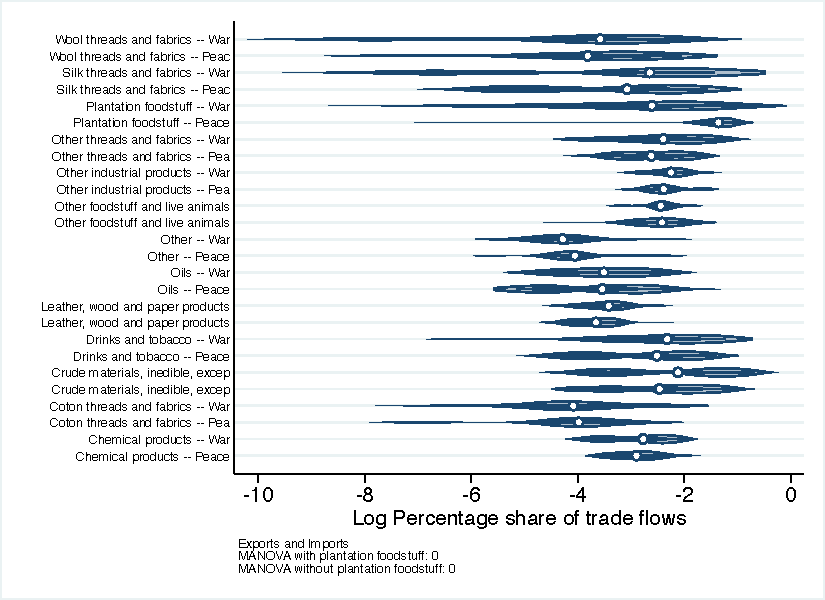
\includegraphics[scale=.7]{peace_war_national_distribution_XI.pdf}
\caption{Distribution of trade Composition}
\label{peace_war_national_distribution_XI}
\end{wrapfigure}
This lead us to take yet another step in the attempt to uncover the underlying mechanisms of trade wars.
We evaluate whether the change in trade structure caused by a war was long lasting, i.e. whether a war changed the structure of trade also for the period after the end of the conflict.
We use a MANOVA test for all the war and peace periods (figure \ref{peace_war_national_distribution_XI}, p-value reported at the bottom) and for each war separately.
The test shows that we can confidently reject the hypothesis that trade composition is unchanged in war versus peace period: that is no surprise.
More interestingly, it shows that after certain wars we fail to reject the hypothesis of a change back and that there is a strong correlation between bigger losses and longer lasting changes in shares of traded products. \\
This has led us to conclude, so far, that the most effective strategy of a trade war was not simply to disrupt trade during the war, but to cause permanent changes in its structure.
We believe that the treatment of neutral trade (which, when possible, allowed French trade to keep its existing structure) and French cooperation (during the blockade period, the French state actively worked to reorient the geography and structure of its trade) were central in achieving this result.



\textbf{Keywords}: international trade, 18th century, France, neutral trade, trade war

%\pagebreak

\renewcommand{\baselinestretch}{1.0}\normalsize
\bibliographystyle{apa}
\bibliography{How_to_wage_a_trade_war}

\end{document}